\documentclass{article}
\usepackage{graphicx} % Required for inserting images

\title{\vspace{-2.5cm}\$SAGE Token Staking Mechanic}
\date{December 2023}

\begin{document}

\maketitle

\section{Asset Income}

The \$SAGE staking contract sources assets used for providing yield from two primary sources.
\begin{itemize}
    \item \subsection{SAGE token buy and sell tax} 
        Whenever SAGE tokens are bought our sold on the open market a 5\% tax is charged.
        Tax collected from token acquisitions is swapped for ETH while the remaining tax stays as SAGE.
        
        From here tokens are split into
        \begin{itemize}
            \item Protocol owned liquidity [20\%]
            \item Protocol treasury [60\%]
            \item Staking contract [20\%]
        \end{itemize}
    \item \subsection{Telesages share trading fee}
        Trading shares on the upcoming Telesages contract generated a trading fee income for the protocol in ETH. This income is added to the SAGE staking contract in full.
\end{itemize}

\begin{figure}[h!]
\centering
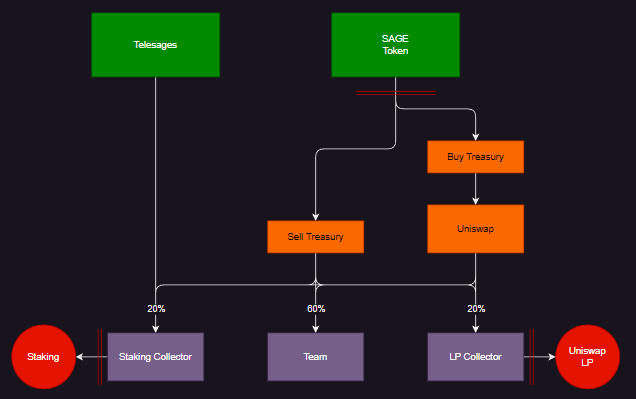
\includegraphics[width=0.75\linewidth]{asset-flow.png}
\caption{SAGE ecosystem revenue flow}
\end{figure}

\section{Staking Model}

\subsection{The "StakePool"}
\label{sec:stakepool}
Assets that are being sent to the Staking contract are distributed to the StakePool instantly or streamed slowly over a given duration.
Each staker receives the as much of a share of the rewards as he hold shares in the StakePool.

\begin{figure}[h!]
\centering
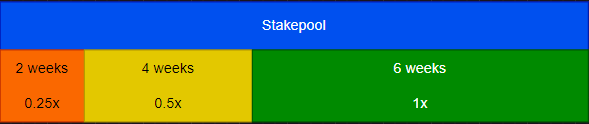
\includegraphics[width=0.75\linewidth]{stakepool.png}
\caption{Stakepool composition example}
\label{fig:stakepool}
\end{figure}

Not all tokens added to the StakePool are weighted equally. Depending on the lockup duration chosen by the staker a certain factor is multiplied to the amount of SAGE staked.

The specific durations and factors available are dynamic and can be changed by the protocol at any time. Changing these values does not however have any effect on historical yield and only applies for all rewards added to the staking contract past the change.

\subsubsection{Example Calculation}
As an example lets consider a StakePool with the lockup-durations shown in \ref{fig:stakepool}.
There are 3 stakers in the pool.
\begin{itemize}
    \item UserA: 1000 SAGE staked for 2 weeks
    \item UserB: 1000 SAGE staked for 4 weeks
    \item UserC: 250 SAGE staked for 6 weeks
\end{itemize}

Now 0.5 ETH of yield is added to the pool without a streaming period (instantly). Based on the duration factors and staked tokens the users will receive:
\begin{itemize}
    \item UserA: 1000 x 0.25 x 0.5 = 0.125 ETH
    \item UserB: 1000 x 0.5 x 0.5 = 0.25 ETH
    \item UserC: 250 x 1 x 0.5 = 0.125 ETH
\end{itemize}

\subsection{Staking}

Staking your SAGE tokens works by sending a transaction calling the respective stake method on the staking contract.
\begin{verbatim}
    function stake(uint256 amount, uint256 duration) external;
\end{verbatim}

This function will transfer the amount of tokens specified in the call from your account to an escrow contract specifically created for each staker. This escrow is used to delegate voting power of the 
staked tokens back to the staker.

\begin{figure}[h!]
\centering
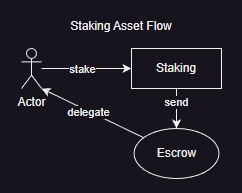
\includegraphics[width=0.5\linewidth]{stake-tx.png}
\caption{Staking transaction flow}
\label{fig:stake-tx-flow}
\end{figure}

Once the tokens are in the escrow the only way to get them back out is by unstaking and withdrawing them. There is no expiry of the stake and no renewal is required.

While the tokens are staked and not pending for unstaking they will be eligible for rewards using the distribution discussed in \ref{sec:stakepool}. Rewards will accrue automatically and do not have an expiry time.

\subsection{Unstaking \& Withdrawing}

If a staker decides to exit the staking contract it's necessary to unstake and withdraw the tokens.
This is the only way for funds to exit the contract.

To do so the staker needs to send an unstake transaction by calling the unstake method on the staking contract.
\begin{verbatim}
    function unstake(uint256 duration) external;
\end{verbatim}

This method will
\begin{itemize}
    \item Claim all outstanding unclaimed rewards
    \item Mark the tokens of the specific staker in the specific lockup-duration as ineligible for rewards
    \item Start a countdown as long as the lockup-duration for withdrawal
\end{itemize}

At this point the staker will have to wait for the full lockup-duration. 
It is not possible to cancel that unstaking process or create a new stake in the same duration that is currently unstaking.
Once the wait time is complete the withdraw method can be called on the staking contract.

\begin{verbatim}
    function withdraw(uint256 duration) external;
\end{verbatim}

This method will transfer all the funds from the escrow contract back to the users wallet
and unblocks the staker from staking new funds in that given lockup-duration.

\section{Claiming / Compounding Rewards}

Rewards in the staking contract cannot expire and do not have any vesting period.
Stakers can decide to claim their outstanding rewards at any time by calling the claim method on the staking contract.

\begin{verbatim}
    function claim(uint256 duration) external;
\end{verbatim}

This will claim rewards for all the reward assets (SAGE, ETH) distributed to the staker
in the given lockup-duration.

\section{Adding rewards / Streaming rewards}
The staking contract supports all ERC20 tokens as well as ETH as staking rewards.
In order to prevent users from adding potential spam or scam reward tokens the reward addition
requires the rewarder to be explicitly whitelisted. This whitelist can be changed at any time by the protocol, see \ref{sec:permissions}.

\subsection{Reward streaming}
When adding a reward to the contract rewarders can specify a duration over which the reward should be streamed to users.
If the duration specified is 0, all rewards will be immediately claimeable by stakers.

However in order to make the yield more predicteable and avoid having to constantly add rewards
it can be beneficial to specify a longer streaming duration instead.

These streamed rewards will be linearily unlocked. That means that after adding the reward at first no rewards can be claimed.
After half of the specified stream durations half of the rewards are claimeable and so on.

Whenever the StakePool (see \ref{sec:stakepool}) changes in size or rewards are claimed, all streaming rewards need to be settled.
This requires going over all running reward streams on-chain.
In order to prevent high gas cost for users it should be avoided to run more than 3 simultaneous reward streams.

\newpage

\section{Administrative access \& Permissions}
\label{sec:permissions}

The staking contract comes with 3 roles / permissions that can be held by other addresses
\begin{itemize}
    \item \subsubsection{Admin}
        Permission to grant roles to other addresses
    \item \subsubsection{Rewarder}
        Permission to add reward tokens / ETH to the contract
    \item \subsubsection{Lockup Manager}
        Permission to change the available lockup-durations as well as their factors
\end{itemize}

\section{Technical Details}
\subsection{Gas efficient reward distribution}
\label{sec:reward-distribution}
Operations on-chain cost gas and can quickly exceed an affordeable range.
In order to be able to distribute rewards to any amount of stakers without having to iterate over all of them an accounting trick is used.

The contract does not store outstanding rewards for each staker but their valuePerShare instead.
Whenever rewards are added to the staking contract, the global valulePerShare is increased.

Whenever a staker claims rewards the outstanding rewards are (simplified):

\begin{verbatim}
    (globalValuePerShare[asset] - lock.valuePerShare[asset]) * tokens * factor
\end{verbatim}

After claiming the lock's valuePerShare will be increased to the global value.

\subsection{Dynamic factor changes}

The mechanism shown in \ref{sec:reward-distribution} breaks down if the factor can dynamically change.
In order to allow changing the factor without having to iterate over all stakers, factor changes create a snapshot of the globalValuePerShare.

When trying to claim reward for a lock that is using a previous factor, the claim will only use the difference till the next factor snapshot.
It will continue going from snapshot to snapshot till the latest is reached again.

This allows for accrued rewards to stay untouched even if a factor is changed.

\end{document}
